\documentclass{article}

% Language setting
% Replace `english' with e.g. `spanish' to change the document language
\usepackage[english]{babel}

% Set page size and margins
% Replace `letterpaper' with `a4paper' for UK/EU standard size
\usepackage[a4paper,top=2cm,bottom=2cm,left=2cm,right=2cm,marginparwidth=1.75cm]{geometry}

\usepackage{amsmath}
\usepackage{ragged2e}
\usepackage{titling}
\usepackage{tikz}
\usepackage{graphicx}
\usepackage{booktabs}
\usepackage[colorlinks=true, allcolors=blue]{hyperref}

\title{\textbf{OT Correction for Self-Consuming Generative Image Models}}

\begin{document}

% === Title ===
\setlength{\droptitle}{-2cm}
\date{}
\maketitle
\vspace*{-2.5cm}


% === Abstract ===
\begin{abstract}
\noindent
Generative models are increasingly trained on data produced by earlier generative
models. When that loop closes on itself, the learned distribution drifts, its tails
disappear, and samples decay towards a small set of prototypes --- \emph{model
collapse} \cite{shumailov2024curse, alemohammad2024selfconsuming}. We study this
process in a self-consuming variational autoencoder (VAE) \cite{kingma2014vae} loop
and evaluate a batch optimal-transport (OT) corrector \cite{gillman2024selfcorrecting}
that, before each new generation trains, transports the synthetic latents back onto a
frozen reference built from real data. Across 40--50 generations on MNIST, Fashion-MNIST and CelebA
we find that (i) an uncorrected loop collapses completely, losing $98\%$ of its
sample diversity by generation $23$; (ii) any correction strength $\lambda > 0$
arrests the collapse, with returns saturating near $\lambda \approx 0.8$; (iii) the
benefit of a larger anchor pool saturates at roughly $10^3$ anchors, indicating that
the transport plan's coverage constraint --- not the number of anchors --- is the
active ingredient; and (iv) the correction generalises across all three datasets. We
also report a negative result: when the full real training set remains available for
augmentation, drift is already suppressed and the corrector adds no further benefit.
The method is therefore best understood as a substitute for real data, not a
supplement to it.
\end{abstract}

% === Contents ===

\section{Correction Methodology}
\subsection{Lambda-Controlled OT Correction}

The corrector operates entirely inside the latent space of a \emph{frozen}
generation-0 VAE. A fixed, class-stratified set of real images is encoded once to
give anchor latents $\{a_j\}$; because neither the encoder nor the anchors are ever
updated, they provide a reference that cannot itself degrade as the loop proceeds.

At generation $k$, the synthetic images are re-encoded by the frozen encoder into
source latents $\{z_i\}$. An optimal-transport plan $P^\star$ is solved between the
uniform empirical measures on the sources and the anchors using the POT library
\cite{flamary2021pot}, and each latent is mapped to its barycentric projection
$T(z_i)$. The correction is applied as a partial move
\begin{equation}
    z_i' \;=\; (1-\lambda)\,z_i \;+\; \lambda\,T(z_i),
    \qquad
    T(z_i) \;=\; \frac{\sum_j P^\star_{ij}\,a_j}{\sum_j P^\star_{ij}},
    \label{eq:blend}
\end{equation}
so that $\lambda$ interpolates between the identity ($\lambda = 0$) and a full
projection onto the anchor manifold ($\lambda = 1$). The corrected latents are
decoded by the frozen decoder and become the training set of generation $k+1$.

The transport polytope constrains \emph{both} marginals: $P\mathbf{1} =
\tfrac{1}{n}\mathbf{1}$ forces every synthetic latent to be corrected, while
$P^{\top}\mathbf{1} = \tfrac{1}{K}\mathbf{1}$ forces every anchor to receive mass.
The second constraint is what distinguishes OT from nearest-neighbour projection, in
which many sources may independently select the same anchor and leave the remainder
of the reference unused.

Solving an exact transport problem against a large anchor pool is intractable, so for
each source chunk we draw a fresh random $K$-subset of the pool and solve exactly
against that subset, resampling per chunk. The cost of each solve scales with $K$
rather than with the pool size, while coverage of the full pool accumulates over the
run \cite{fatras2020minibatch}. Coverage is therefore enforced exactly \emph{within}
each subset and only statistically across the pool; minibatch OT is also a biased
estimator of the full-pool plan, and we do not claim the two are equivalent.

\begin{figure}[h!]
    \centering
    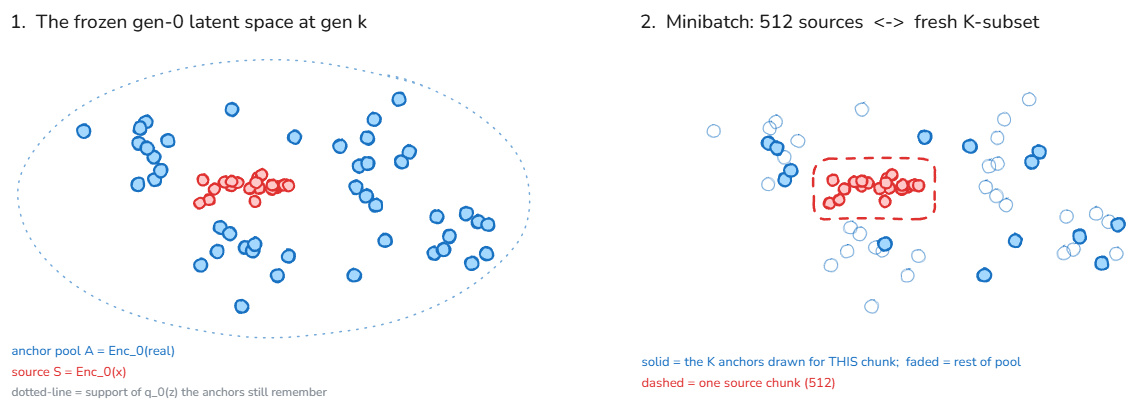
\includegraphics[width=0.8\linewidth]{Images/ot_pipeline_1.png}
    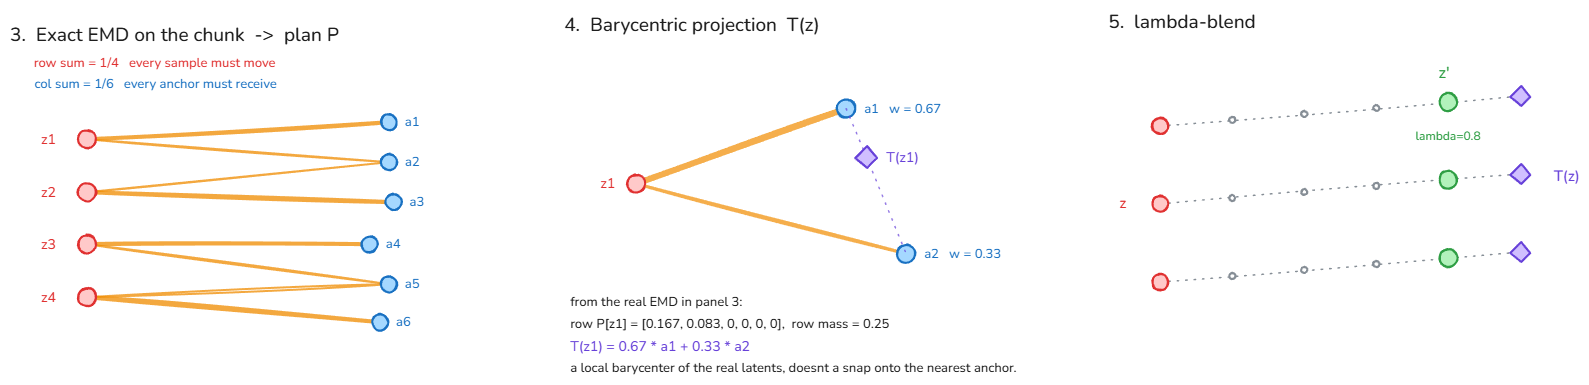
\includegraphics[width=1\linewidth]{Images/ot_pipeline_2.png}
    \caption{The correction operator. \textbf{Top:} the frozen generation-0 latent
    space at generation $k$ --- the anchor cloud (blue) is fixed, while the
    re-encoded synthetic cloud (red) has contracted towards the high-density core;
    minibatch OT pairs one chunk of sources with a freshly drawn $K$-subset of the
    anchor pool. \textbf{Bottom:} the exact transport plan on that chunk, whose line
    thickness is the transported mass $P_{ij}$; the barycentric projection $T(z)$
    formed as a convex combination of the anchors a latent transports to; and the
    $\lambda$-blend of Equation~\eqref{eq:blend} that produces the latent which is
    finally decoded.}
    \label{fig:pipeline}
\end{figure}

\subsection{Self-Consuming VAE}

Each generation trains a fresh VAE from scratch on the previous generation's output,
so no parameters are carried forward and the only channel between generations is the
data itself. Generation 0 trains on a $10{,}000$-image sample of the real training
set; every later generation trains on $10{,}000$ synthetic images produced by its
predecessor.

\begin{figure}[h!]
    \centering
    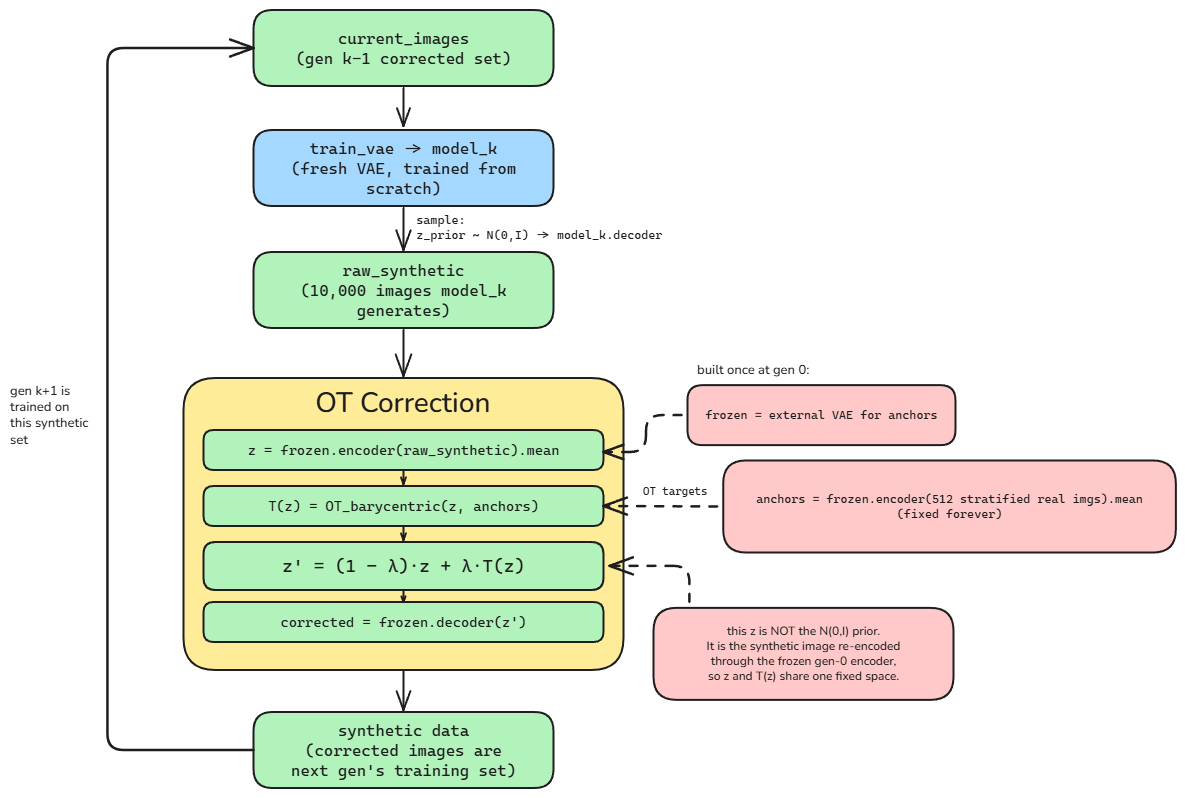
\includegraphics[width=5in]{Images/self_consuming.png}
    \caption{One iteration of the self-consuming loop with OT correction. The frozen
    generation-0 VAE and its anchor latents are built once and reused thereafter; the
    latents entering the corrector are synthetic images re-encoded through that frozen
    encoder, not draws from the $\mathcal{N}(0, I)$ prior, so sources and anchors
    share a single fixed coordinate system.}
    \label{fig:loop}
\end{figure}

\subsection{Evaluation}

We report three measures per generation, all computed against fixed references so
that they remain comparable as the loop proceeds:

\begin{itemize}
    \item \textbf{Distributional drift.} The sliced Wasserstein distance
    ($W_2$, 100 projections) between the current generation's prior samples and
    generation 0's, in a fixed feature space. This is our headline metric: it is zero
    by construction at generation 0 and grows as the model departs from its starting
    distribution. Features come from a small CNN trained on the dataset itself for
    MNIST and Fashion-MNIST, and from a self-contained pixel-pooling embedding for
    CelebA. Absolute values are therefore comparable \emph{within} a dataset but not
    \emph{across} datasets.
    \item \textbf{Sample diversity.} The mean per-pixel standard deviation across a
    batch of samples, which falls towards zero as the model collapses onto a
    prototype.
    \item \textbf{Reconstruction error.} Binary cross-entropy on a held-out set of
    \emph{real} test images, measuring how well the generation-$k$ model still
    explains real data.
\end{itemize}

\pagebreak
\section{Results}

\subsection{Qualitative Collapse}

\begin{figure}[h!]
\centering
\begin{tikzpicture}[picture format/.style={inner sep=2pt,}]

  \node[picture format]                   (A1)               {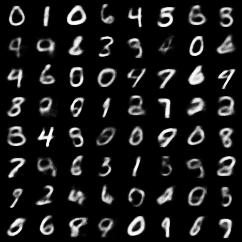
\includegraphics[width=1.25in]{Images/VAE_baseline/mnist_g0_samples.png}};
  \node[picture format,anchor=north]      (B1) at (A1.south) {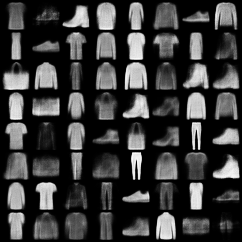
\includegraphics[width=1.25in]{Images/VAE_baseline/fashion_g0_samples.png}};
  \node[picture format,anchor=north]      (C1) at (B1.south) {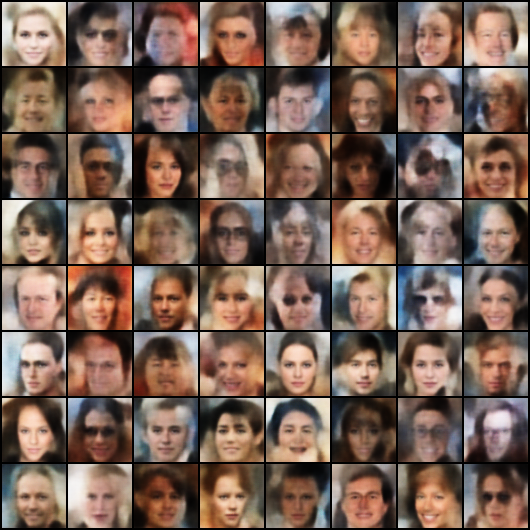
\includegraphics[width=1.25in]{Images/VAE_baseline/celeba_g0_samples.png}};

  \node[picture format,anchor=north west] (A2) at (A1.north east) {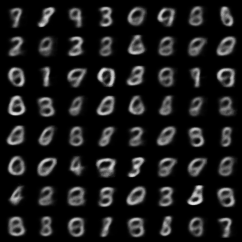
\includegraphics[width=1.25in]{Images/VAE_baseline/mnist_g10_samples.png}};
  \node[picture format,anchor=north]      (B2) at (A2.south)      {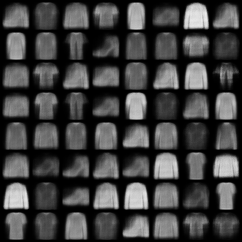
\includegraphics[width=1.25in]{Images/VAE_baseline/fashion_g10_samples.png}};
  \node[picture format,anchor=north]      (C2) at (B2.south) {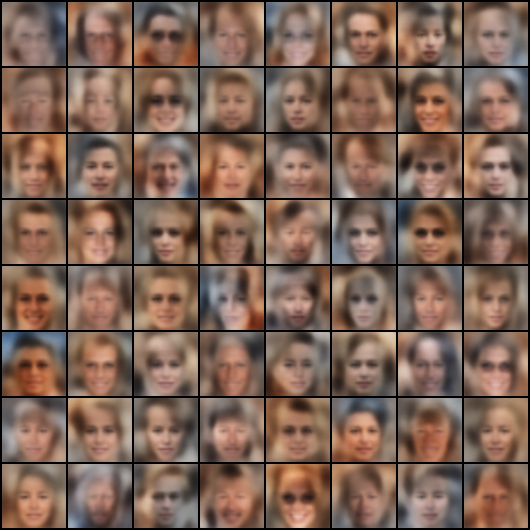
\includegraphics[width=1.25in]{Images/VAE_baseline/celeba_g10_samples.png}};

  \node[picture format,anchor=north west] (A3) at (A2.north east) {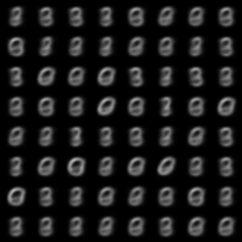
\includegraphics[width=1.25in]{Images/VAE_baseline/mnist_g20_samples.png}};
  \node[picture format,anchor=north]      (B3) at (A3.south)      {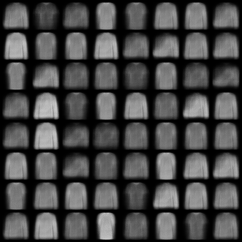
\includegraphics[width=1.25in]{Images/VAE_baseline/fashion_g20_samples.png}};
  \node[picture format,anchor=north]      (C3) at (B3.south) {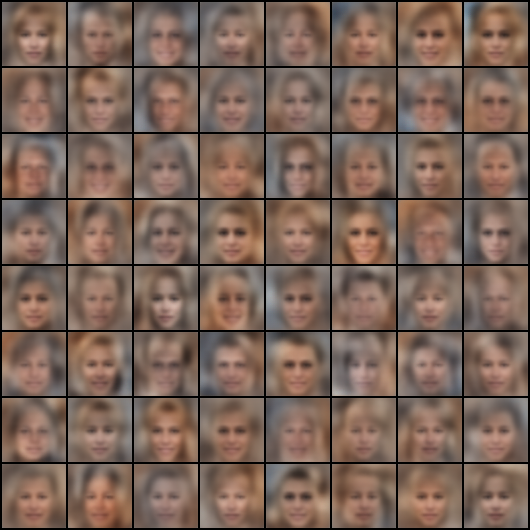
\includegraphics[width=1.25in]{Images/VAE_baseline/celeba_g20_samples.png}};

  \node[picture format,anchor=north west] (A4) at (A3.north east) {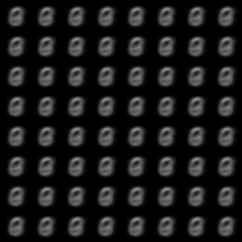
\includegraphics[width=1.25in]{Images/VAE_baseline/mnist_g30_samples.png}};
  \node[picture format,anchor=north]      (B4) at (A4.south)      {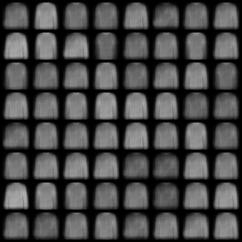
\includegraphics[width=1.25in]{Images/VAE_baseline/fashion_g30_samples.png}};
  \node[picture format,anchor=north]      (C4) at (B4.south) {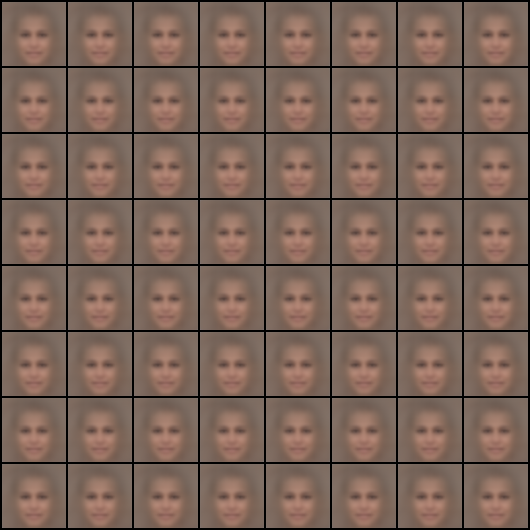
\includegraphics[width=1.25in]{Images/VAE_baseline/celeba_g30_samples.png}};

  %% Captions
  \node[anchor=north] (D1) at (C1.south) {\bfseries Gen. 0};
  \node[anchor=north] (D2) at (C2.south) {\bfseries Gen. 10};
  \node[anchor=north] (D3) at (C3.south) {\bfseries Gen. 20};
  \node[anchor=north] (D4) at (C4.south) {\bfseries Gen. 30};

\end{tikzpicture}
\caption{MNIST, Fashion-MNIST, CelebA synthetic samples at $i$th generation VAE after training on 10000 fully synthetic samples generated from $i - 1$th generation. Generation 0 was trained on a 10000 image sample of the real training datasets.}
\label{fig:qual-baseline}
\end{figure}


\begin{figure}[h!]
\centering
\begin{tikzpicture}[picture format/.style={inner sep=2pt,}]

  \node[picture format]                   (A1)               {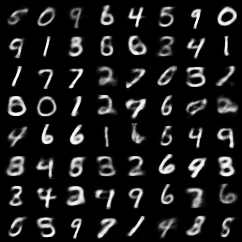
\includegraphics[width=1.25in]{Images/VAE_ot/ot_mnist_g0.png}};
  \node[picture format,anchor=north]      (B1) at (A1.south) {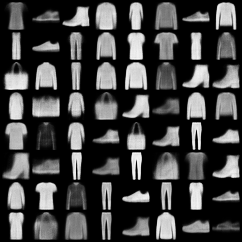
\includegraphics[width=1.25in]{Images/VAE_ot/ot_fashion_g0.png}};
  \node[picture format,anchor=north]      (C1) at (B1.south) {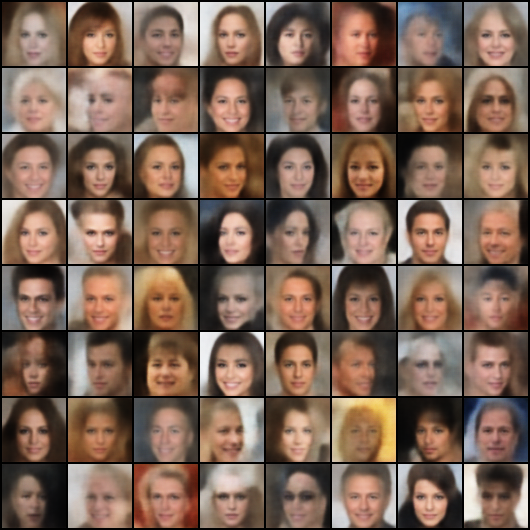
\includegraphics[width=1.25in]{Images/VAE_ot/ot_celeba_g0.png}};

  \node[picture format,anchor=north west] (A2) at (A1.north east) {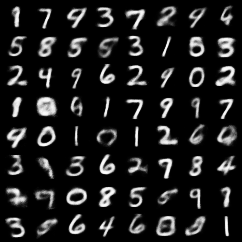
\includegraphics[width=1.25in]{Images/VAE_ot/ot_mnist_g10.png}};
  \node[picture format,anchor=north]      (B2) at (A2.south)      {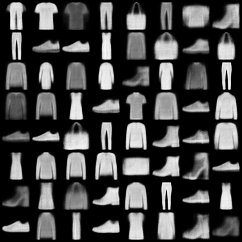
\includegraphics[width=1.25in]{Images/VAE_ot/ot_fashion_g10.png}};
  \node[picture format,anchor=north]      (C2) at (B2.south) {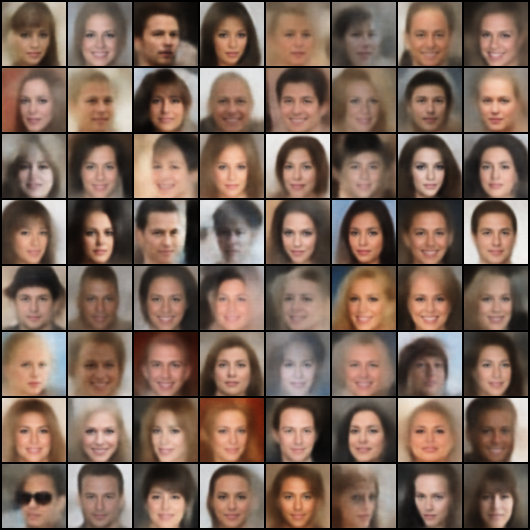
\includegraphics[width=1.25in]{Images/VAE_ot/ot_celeba_g10.png}};

  \node[picture format,anchor=north west] (A3) at (A2.north east) {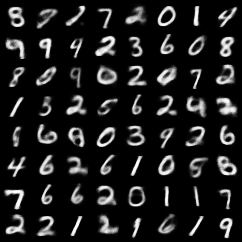
\includegraphics[width=1.25in]{Images/VAE_ot/ot_mnist_g20.png}};
  \node[picture format,anchor=north]      (B3) at (A3.south)      {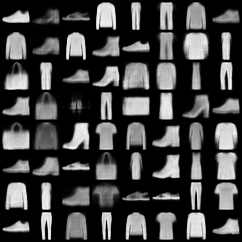
\includegraphics[width=1.25in]{Images/VAE_ot/ot_fashion_g20.png}};
  \node[picture format,anchor=north]      (C3) at (B3.south) {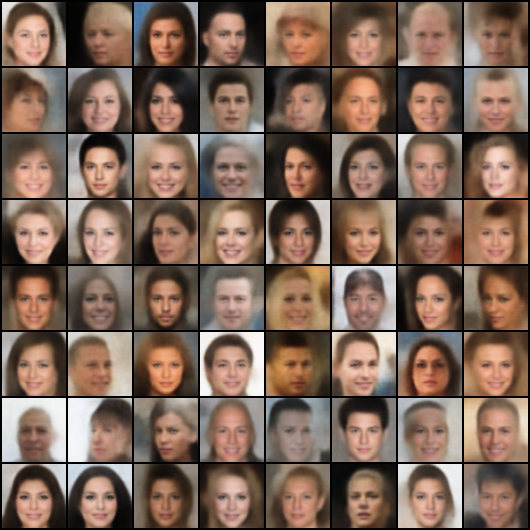
\includegraphics[width=1.25in]{Images/VAE_ot/ot_celeba_g20.png}};

  \node[picture format,anchor=north west] (A4) at (A3.north east) {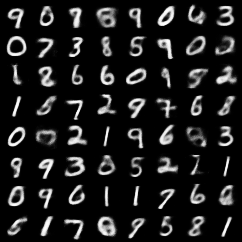
\includegraphics[width=1.25in]{Images/VAE_ot/ot_mnist_g30.png}};
  \node[picture format,anchor=north]      (B4) at (A4.south)      {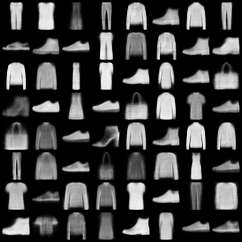
\includegraphics[width=1.25in]{Images/VAE_ot/ot_fashion_g30.png}};
  \node[picture format,anchor=north]      (C4) at (B4.south) {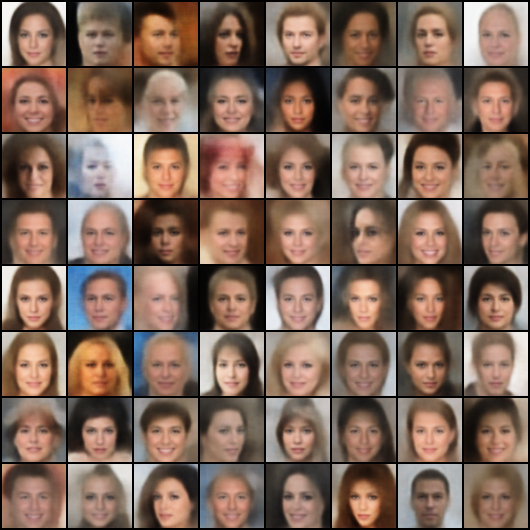
\includegraphics[width=1.25in]{Images/VAE_ot/ot_celeba_g30.png}};

  %% Captions
  \node[anchor=north] (D1) at (C1.south) {\bfseries Gen. 0};
  \node[anchor=north] (D2) at (C2.south) {\bfseries Gen. 10};
  \node[anchor=north] (D3) at (C3.south) {\bfseries Gen. 20};
  \node[anchor=north] (D4) at (C4.south) {\bfseries Gen. 30};

\end{tikzpicture}
\caption{MNIST, Fashion-MNIST, CelebA OT-corrected synthetic samples at $i$th generation VAE after training on 10000 fully synthetic samples generated from $i - 1$th generation. No OT regularisation, $\lambda = 0.8$, 10000 randomly chosen anchor images.}
\label{fig:qual-ot}
\end{figure}

Figures~\ref{fig:qual-baseline} and~\ref{fig:qual-ot} show the effect qualitatively.
Without correction, all three datasets lose variety as the generations compound: the
MNIST digits thicken and converge towards a common stroke, the Fashion-MNIST garments
merge into a single silhouette, and the CelebA faces converge to a near-identical
frontal portrait. With $\lambda = 0.8$, samples at generation 30 remain visibly as
varied as at generation 0.

\pagebreak
\subsection{Varying Anchor Size \& Barycentric Strength \texorpdfstring{$\lambda$}{lambda}}

We sweep the two parameters of the corrector independently on MNIST, holding all
other settings fixed ($10{,}000$ images per generation, 40 epochs, 40 generations).
The correction-strength sweep uses $5{,}000$ anchors with exact transport; the anchor
sweep fixes $\lambda = 0.8$ and uses minibatch OT with $K = 1000$.

\begin{figure}[h!]
    \centering
    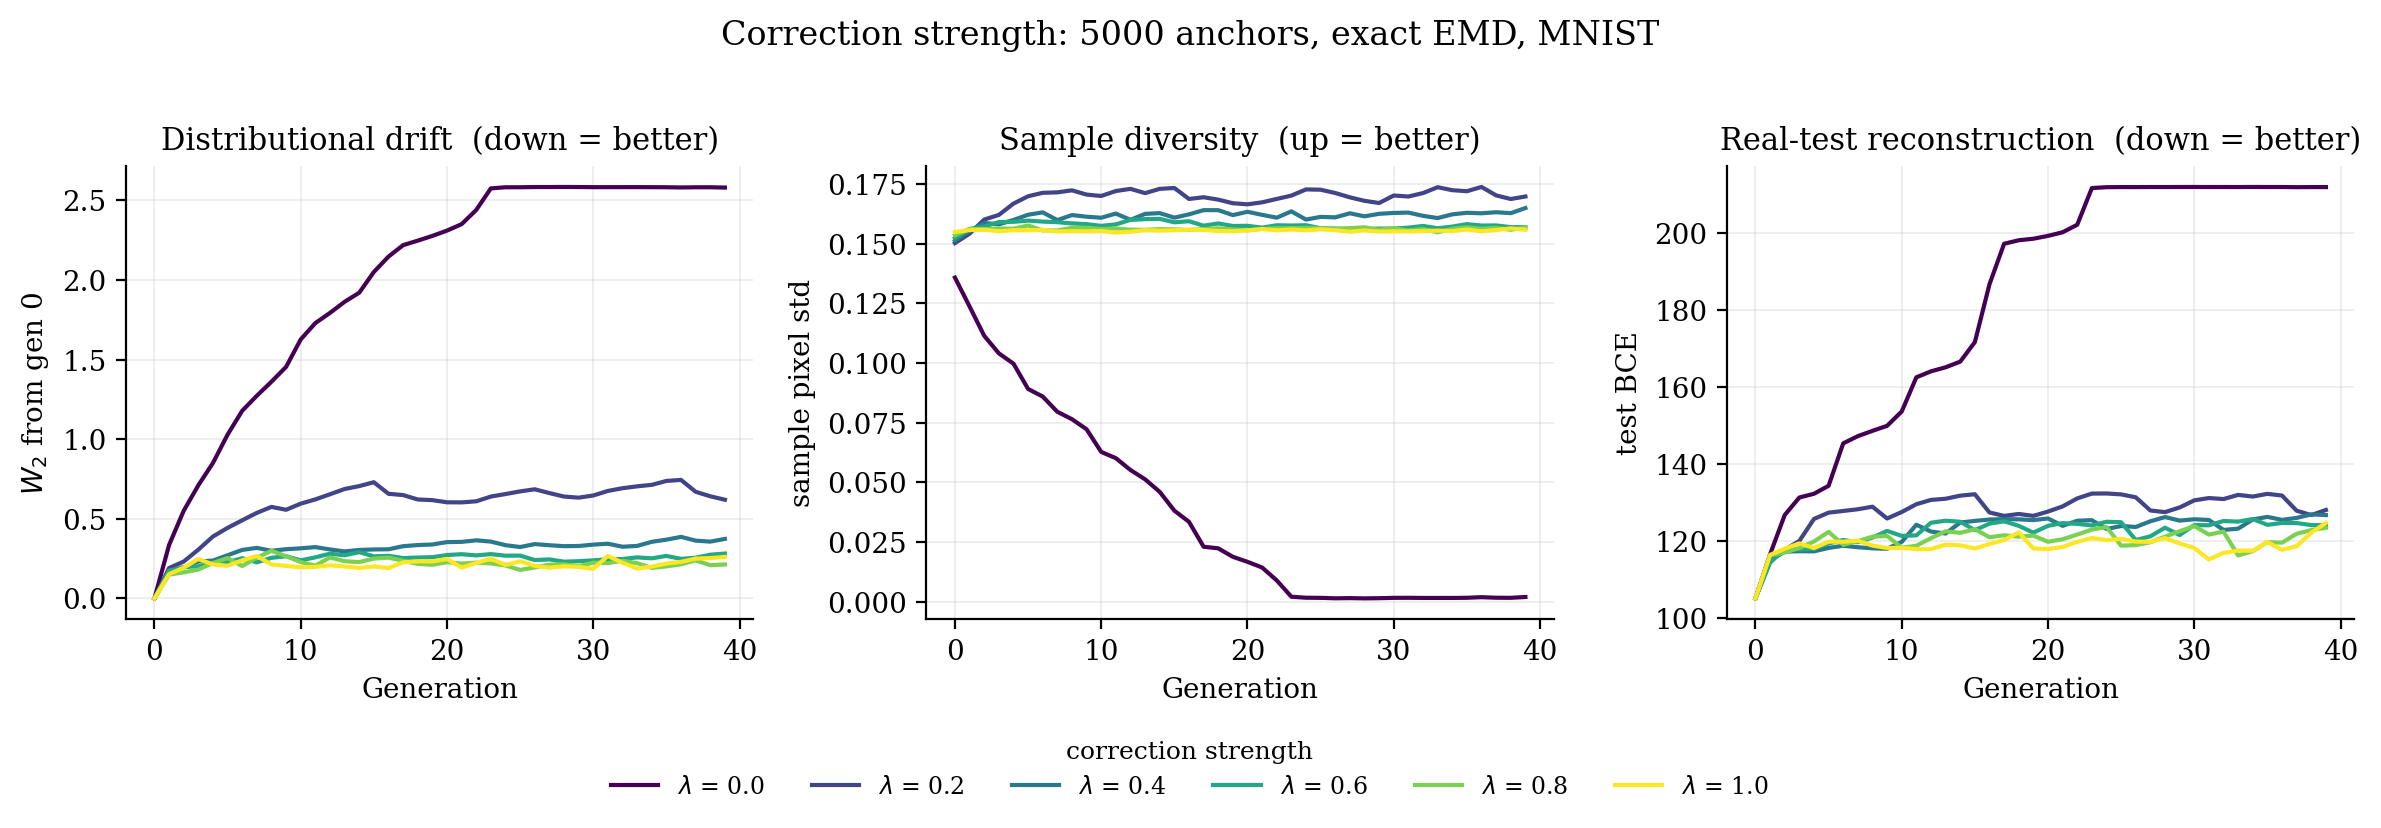
\includegraphics[width=\linewidth]{Images/results/lambda_sweep.png}
    \caption{Correction strength $\lambda$, all runs overlaid. The uncorrected loop
    ($\lambda = 0$) drifts monotonically until generation $23$, at which point it has
    collapsed onto a single prototype and the curves flatten: diversity is pinned near
    zero and no further change is possible. Every $\lambda > 0$ arrests the collapse,
    and the improvement is strongly diminishing --- most of the benefit is already
    obtained by $\lambda = 0.4$.}
    \label{fig:lambda}
\end{figure}

\begin{table}[h!]
\centering
\caption{Correction strength, mean over the final 10 generations. Best value per
column in bold. Generation-0 reference: BCE $= 105.1$.}
\label{tab:lambda}
\begin{tabular}{lccc}
\toprule
$\lambda$ & $W_2$ from gen 0 $\downarrow$ & Sample diversity $\uparrow$ & Test BCE $\downarrow$ \\
\midrule
0.0 (uncorrected) & 2.583 & 0.002 & 211.8 \\
0.2 & 0.684 & \textbf{0.171} & 130.2 \\
0.4 & 0.354 & 0.163 & 125.4 \\
0.6 & 0.257 & 0.157 & 124.5 \\
0.8 & \textbf{0.217} & 0.156 & 120.9 \\
1.0 & 0.227 & 0.156 & \textbf{118.8} \\
\bottomrule
\end{tabular}
\end{table}

Table~\ref{tab:lambda} quantifies the trade-off. Drift falls steeply from
$\lambda = 0$ to $\lambda = 0.4$ and then flattens, reaching its minimum at
$\lambda = 0.8$; the marginal gain from $0.6$ to $0.8$ is $0.04$ in $W_2$, against
$2.23$ for the first step away from zero. Reconstruction error improves monotonically
in $\lambda$, while diversity is highest at the \emph{weakest} nonzero correction and
declines slightly thereafter --- at large $\lambda$ the samples increasingly resemble
decoded anchor barycentres, which are smoother than the model's own output. No single
$\lambda$ optimises all three measures, but $\lambda \in [0.6, 1.0]$ is a broad
plateau in which all three are close to their best values, and we use $\lambda = 0.8$
elsewhere in this report.

\begin{figure}[h!]
    \centering
    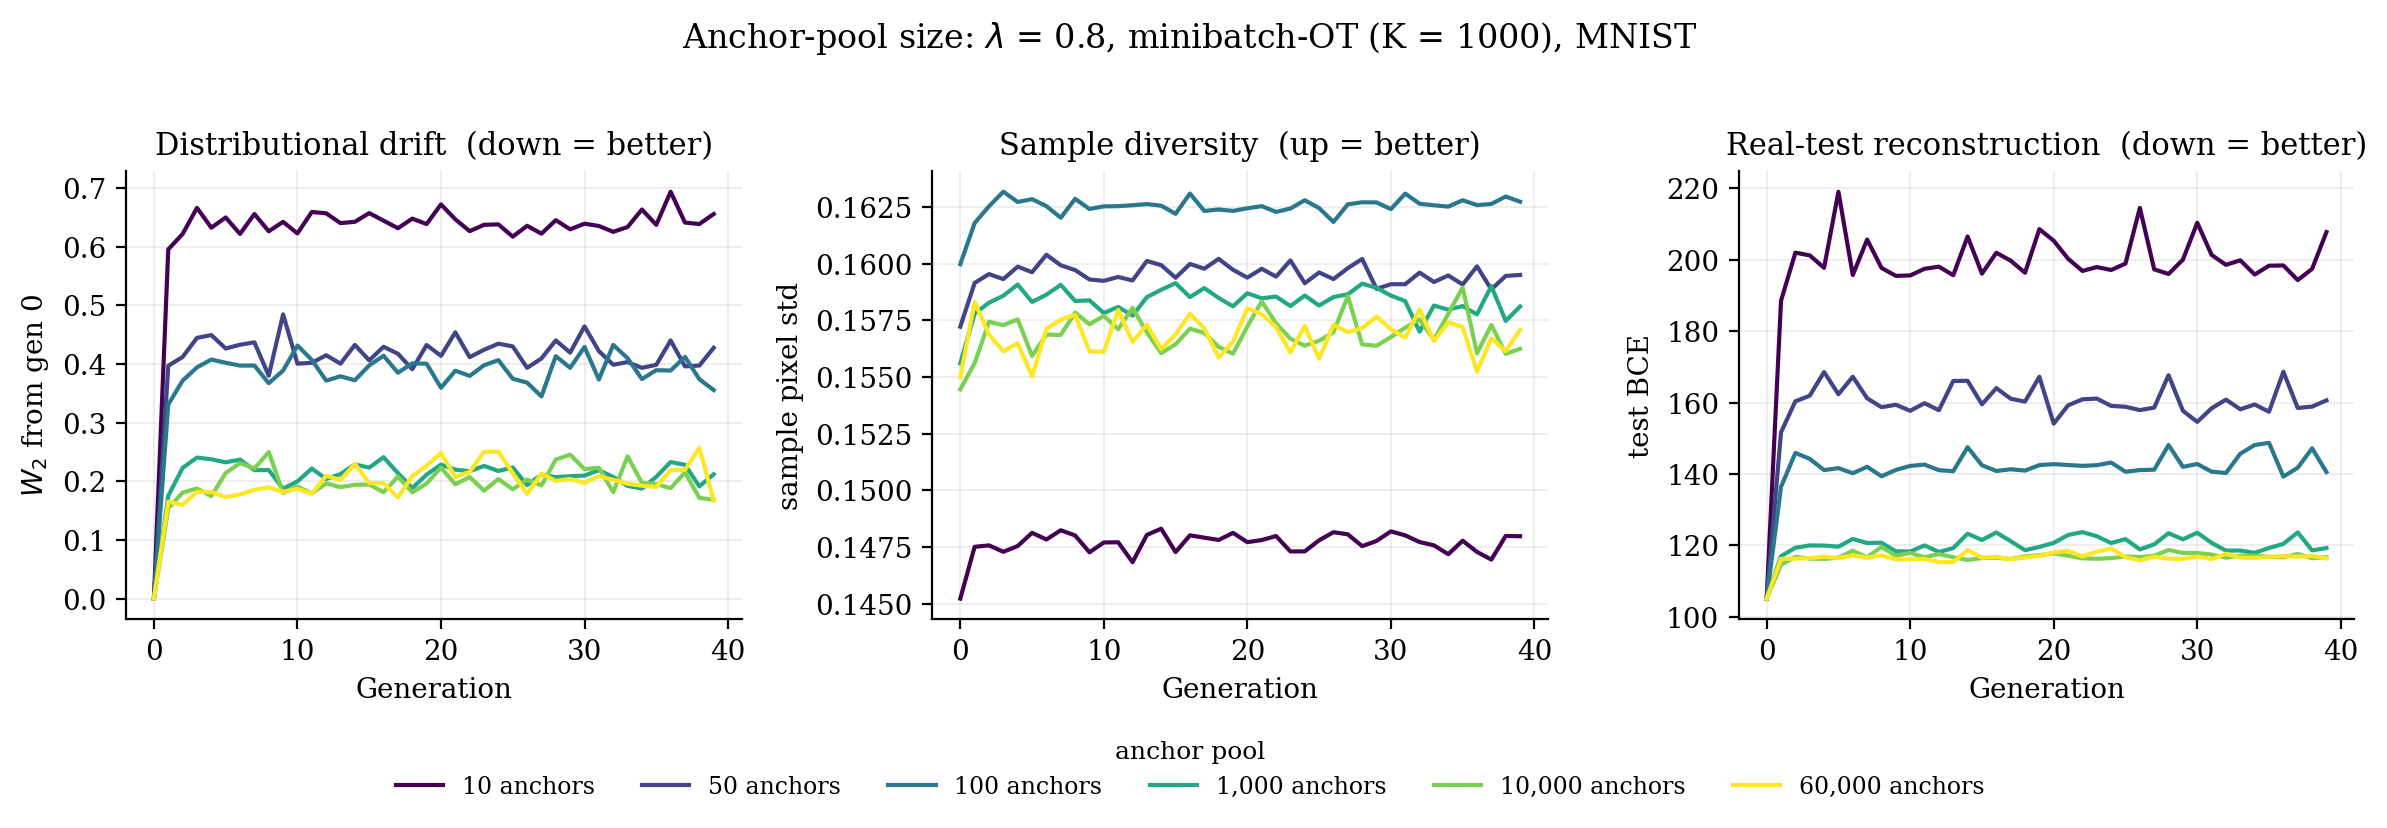
\includegraphics[width=\linewidth]{Images/results/anchor_sweep.png}
    \caption{Anchor-pool size at $\lambda = 0.8$, all runs overlaid. Increasing the
    pool from 10 to $1{,}000$ anchors reduces drift by two thirds; increasing it a
    further sixty-fold changes nothing measurable. Note that no configuration
    collapses --- even 10 anchors hold the loop stable, in contrast to the uncorrected
    run of Figure~\ref{fig:lambda}.}
    \label{fig:anchors}
\end{figure}

\begin{table}[h!]
\centering
\caption{Anchor-pool size at $\lambda = 0.8$, mean over the final 10 generations.}
\label{tab:anchors}
\begin{tabular}{lccc}
\toprule
Anchors & $W_2$ from gen 0 $\downarrow$ & Sample diversity $\uparrow$ & Test BCE $\downarrow$ \\
\midrule
10 & 0.646 & 0.148 & 200.2 \\
50 & 0.414 & 0.159 & 159.5 \\
100 & 0.394 & \textbf{0.163} & 143.5 \\
1{,}000 & 0.209 & 0.158 & 120.0 \\
10{,}000 & \textbf{0.200} & 0.157 & 117.0 \\
60{,}000 & 0.205 & 0.157 & \textbf{116.7} \\
\bottomrule
\end{tabular}
\end{table}

The saturation in Table~\ref{tab:anchors} is the more informative result. Between
$1{,}000$ and $60{,}000$ anchors --- a sixty-fold increase in the amount of real data
the corrector sees --- drift changes by $0.004$, which is within the run-to-run
fluctuation visible in Figure~\ref{fig:anchors}. This is consistent with the
barycentric projection of Equation~\eqref{eq:blend} being a \emph{local} average: with
a source chunk of $n$ points and $K$ anchors, the marginal constraint forces each
source to spread its mass over at least $\lceil K/n \rceil$ anchors, so the
averaging neighbourhood is set by the chunk size rather than by the pool. Additional
anchors resolve the same local conditional mean more finely; they do not enlarge it.
What matters is that the plan is forced to cover whatever reference it is given, and
even a very small reference is sufficient to stop the loop from collapsing.

\pagebreak
\subsection{Data Augmentation and Corrected Augmentation}

The experiments above replace the training set entirely with synthetic data, which is
the worst case. In practice a self-consuming loop may retain access to some real data,
and accumulating rather than replacing data is itself known to mitigate collapse
\cite{gerstgrasser2024accumulate}.
We therefore compare four regimes on MNIST, all at 60 epochs per generation: pure
synthetic replacement; retaining a fixed set of $512$ real images in each generation's
training set; augmenting each generation with the \emph{full} real pool; and that same
full augmentation combined with correction.

\begin{figure}[h!]
    \centering
    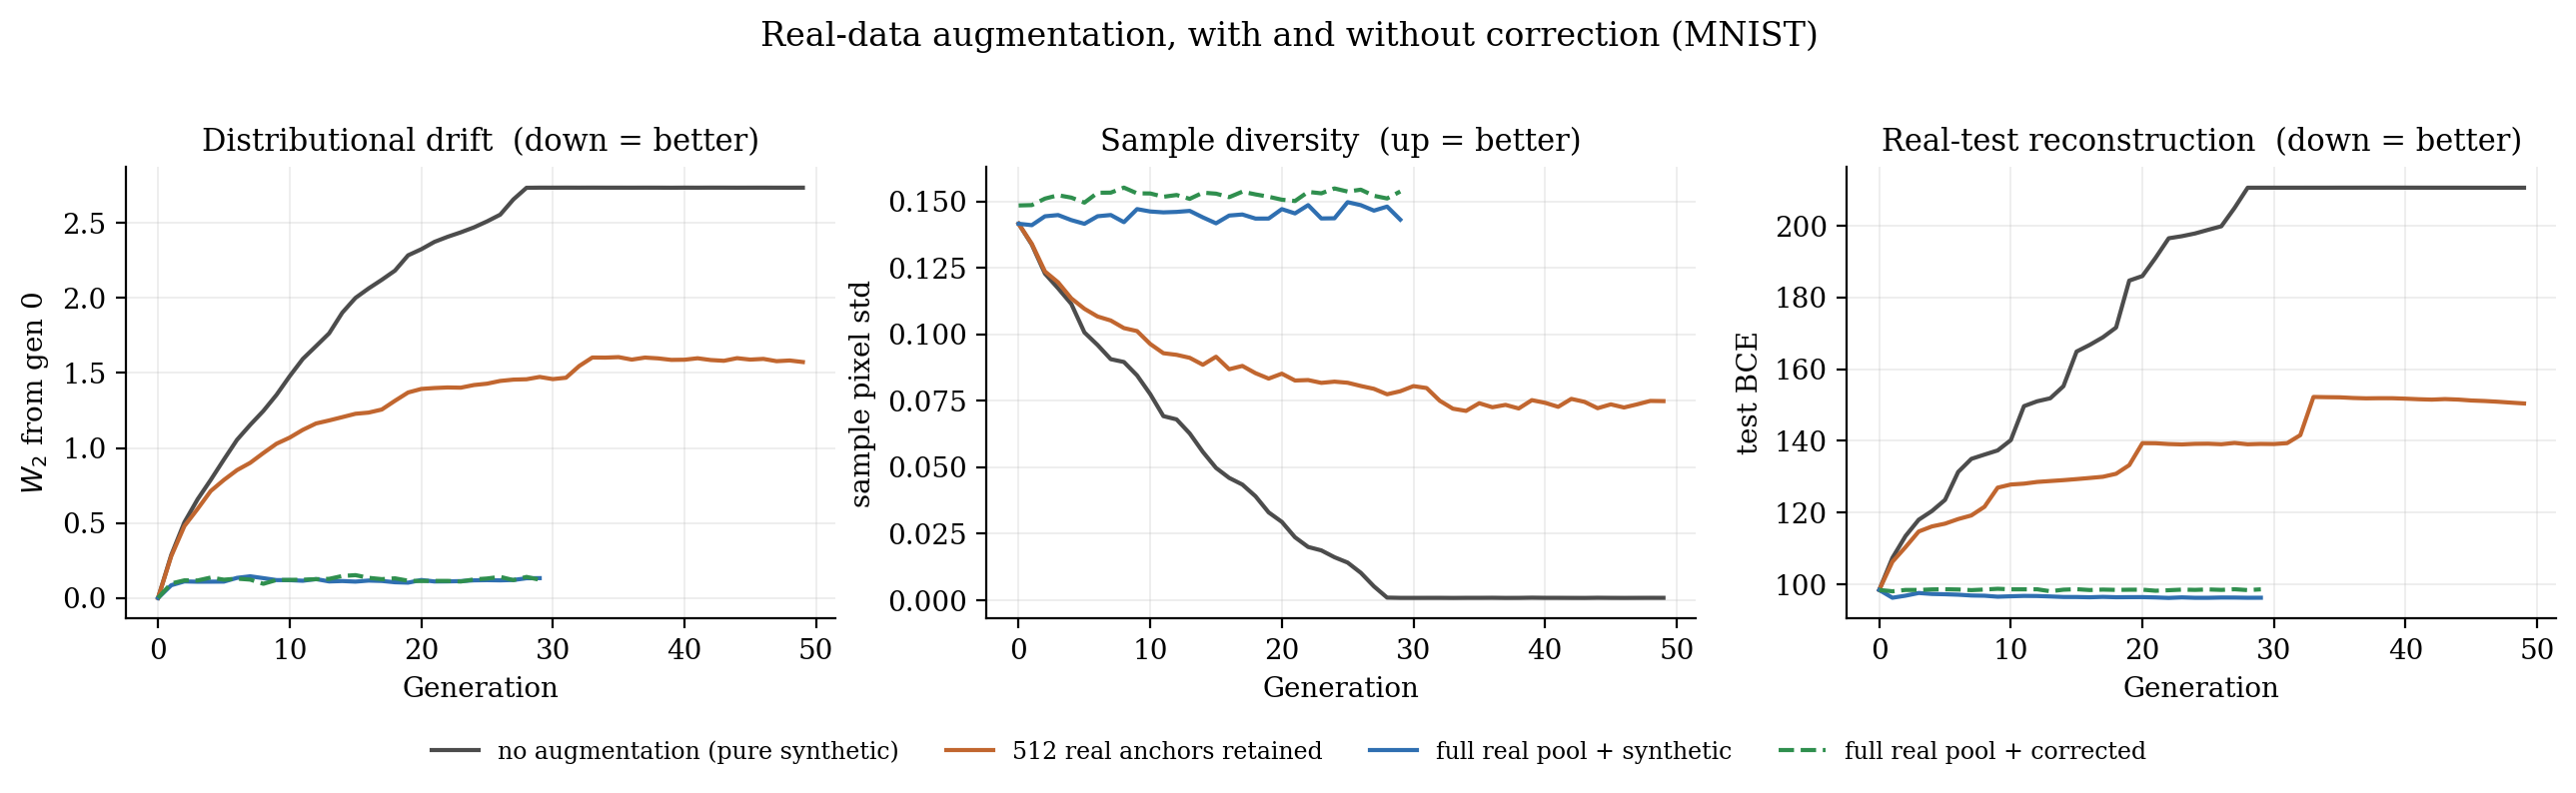
\includegraphics[width=\linewidth]{Images/results/augmentation.png}
    \caption{Real-data augmentation with and without correction. The two augmented
    runs are almost indistinguishable, and both are far below the two unaugmented
    runs. Note that the corrected run uses nearest-neighbour projection onto a
    512-anchor bank at $\lambda = 1.0$ rather than the barycentric OT corrector used
    elsewhere; the augmented runs terminate at generation 30.}
    \label{fig:augmentation}
\end{figure}

\begin{table}[h!]
\centering
\caption{Augmentation regimes, mean over the final 5 generations of each run.}
\label{tab:augmentation}
\begin{tabular}{lccc}
\toprule
Regime & $W_2$ from gen 0 $\downarrow$ & Sample diversity $\uparrow$ & Test BCE $\downarrow$ \\
\midrule
Pure synthetic (no augmentation) & 2.735 & 0.001 & 210.5 \\
$512$ real images retained & 1.583 & 0.074 & 150.9 \\
Full real pool $+$ synthetic & \textbf{0.124} & 0.147 & \textbf{96.3} \\
Full real pool $+$ corrected & 0.130 & \textbf{0.153} & 98.5 \\
\bottomrule
\end{tabular}
\end{table}

Two results stand out. First, retaining $512$ real \emph{images} in the training set
slows collapse but does not prevent it: drift still reaches $1.58$ and diversity falls
by half. This contrasts sharply with using the same number of real images as OT
\emph{anchors}, which holds drift near $0.2$ indefinitely. The difference is not the
quantity of real data but how it is used --- as a small minority of the training
signal it is simply outvoted, whereas as a transport target it constrains every
synthetic sample.

Second, and less favourably for the method, once the full real pool is retained the
corrector adds nothing. The augmented and corrected-augmented runs differ by $0.006$
in $W_2$ and $2.2$ in BCE, in opposite directions, which is well inside run-to-run
variation; the corrected run has marginally higher diversity and marginally worse
reconstruction. Abundant real data already pins the distribution in place, and there
is no residual drift for the corrector to remove. We therefore read the corrector as a
\emph{substitute} for real data in the regime where it is scarce or unavailable, not
as a supplement that improves on having it. We note two caveats on this comparison:
the corrected run used nearest-neighbour projection at $\lambda = 1.0$ rather than the
barycentric corrector characterised in Section 2.1, and both augmented runs were
stopped at generation 30, so we cannot rule out a divergence appearing later.

\subsection{Generality Across Datasets}

Finally we check that the correction is not specific to MNIST. Figure~\ref{fig:cross}
compares the drift trajectory of the corrected and uncorrected loops on all three
datasets at $\lambda = 0.8$.

\begin{figure}[h!]
    \centering
    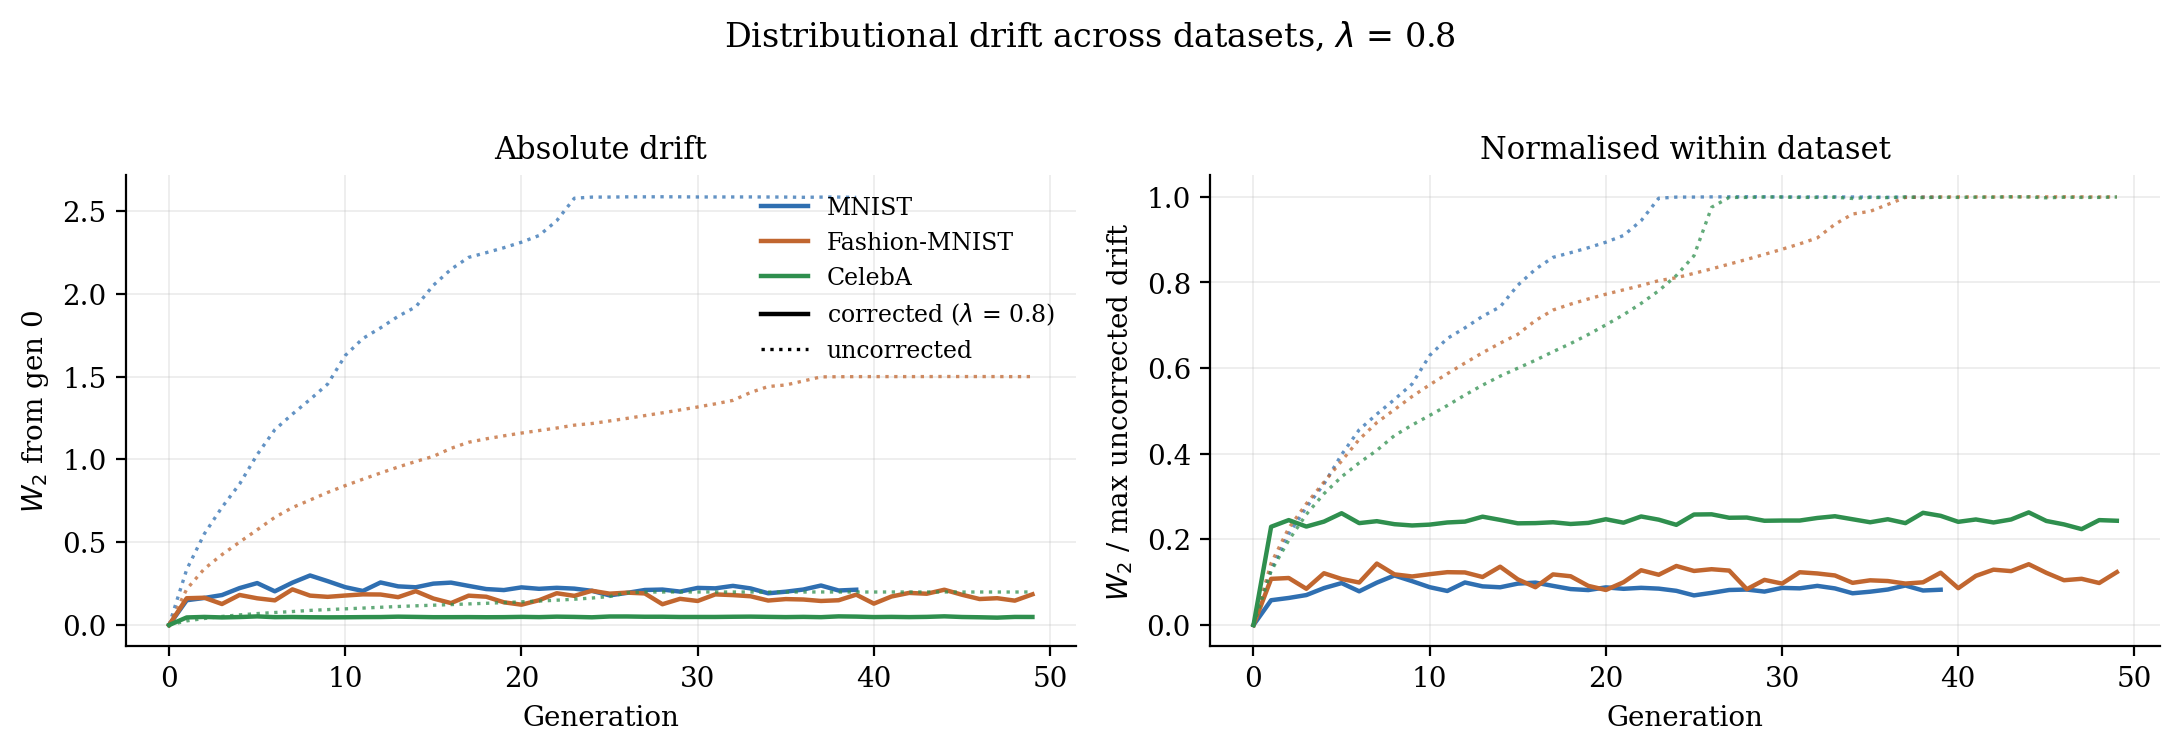
\includegraphics[width=\linewidth]{Images/results/cross_dataset.png}
    \caption{Drift with and without correction on three datasets. \textbf{Left:}
    absolute $W_2$. Because each dataset uses its own feature space, the vertical
    scales are not comparable between datasets --- only the shape of each pair of
    curves is. \textbf{Right:} the same curves with each dataset normalised by the
    maximum drift of its own uncorrected run, which makes the relative effect
    comparable.}
    \label{fig:cross}
\end{figure}

\begin{table}[h!]
\centering
\caption{Final-generation drift, corrected ($\lambda = 0.8$) versus uncorrected.}
\label{tab:cross}
\begin{tabular}{lccc}
\toprule
Dataset & Uncorrected $W_2$ & Corrected $W_2$ & Fraction retained \\
\midrule
MNIST & 2.581 & 0.213 & 0.08 \\
Fashion-MNIST & 1.500 & 0.185 & 0.12 \\
CelebA & 0.200 & 0.049 & 0.24 \\
\bottomrule
\end{tabular}
\end{table}

The pattern is consistent: on all three datasets the uncorrected loop drifts steadily
until it saturates, while the corrected loop rises briefly and then holds a flat
plateau for the remainder of the run. The corrected loop retains between $8\%$ and
$24\%$ of the uncorrected drift. The CelebA ratio is the least favourable, but it is
also the least directly comparable: CelebA drift is measured in a pixel-pooling
feature space that is deliberately insensitive to the high-frequency detail a VAE
loses first, so its uncorrected baseline has a much smaller dynamic range to begin
with, and the ratio is correspondingly compressed. The qualitative samples of
Figure~\ref{fig:qual-baseline} make the CelebA collapse obvious even where this
metric understates it.

\section{Conclusion}

A self-consuming VAE loop collapses completely within roughly $25$ generations,
losing essentially all sample diversity. Transporting each generation's latents back
onto a frozen reference of real anchors prevents this, and does so robustly: any
$\lambda > 0$ arrests the collapse, and even $10$ anchors are sufficient to keep the
loop stable, though $\lambda \approx 0.8$ with $\gtrsim 10^3$ anchors is where the
measured optimum sits. The saturation in anchor count, together with the large gap
between using $512$ real images as anchors and using the same images as training data,
supports the interpretation that the operative mechanism is the transport plan's
coverage constraint rather than the volume of real data supplied.

The method's limits are equally clear. It does not improve on simply retaining real
training data when that data is available, and our augmentation comparison used a
nearest-neighbour variant over a shorter run, so a direct barycentric comparison at
matched length remains to be done. Minibatch OT, which we rely on for large pools,
enforces coverage only within each drawn subset and is a biased estimator of the
full-pool plan. Finally, all results here use a single architecture at one scale; we
have not tested whether the same correction transfers to stronger generative families
where the collapse dynamics may differ.

\bibliographystyle{plain}
\bibliography{sample}

\end{document}
